\subsubsection{Proximity analysis}\label{rooms}
This section describes a simple method (proximity analysis) of performing localization using radio-based hardware.
The technique, as described in \citet[Section II.C Proximity]{wireless_survey}, works by determining if the item being located is within the range of one or more fixed antennas with known locations.
If the item is within the range of a single antenna, its location is said to be that of the antenna.
If the item is within the range of multiple antennas, its location is said to be that of the antenna with the greatest signal strength.

In \cref{rooms:fig:cover} are three rooms $R_1$, $R_2$ and $R_3$ that are fitted with low range radio-based antennas.
Rooms $R_1$ and $R_2$ have been fitted with antennas to allow for the localization whereas $R_3$ only has preexisting antennas.

\begin{figure}[h]
\centering
\tikzstyle{rfid}=[draw=none, fill=blue, fill opacity=0.7, text opacity=1, circle, minimum size=0.6cm]
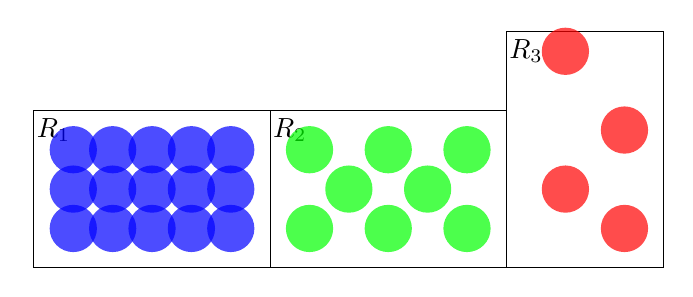
\begin{tikzpicture}[scale=0.5]

\draw  (-6,0) rectangle (-12,4);
\node at (-11.5,3.5) {$R_1$};

\draw  (0,0) rectangle (-6,4);
\node at (-5.5,3.5) {$R_2$};

\draw  (0,0) rectangle (4,6);
\node at (0.5,5.5) {$R_3$};

\def \n {5}
\def \radius {3cm}
\def \margin {8} % margin in angles, depends on the radius

\foreach \x in {0,...,4}{\foreach \y in {0,...,2}{
  \node[rfid] at (-11 + \x,3 - \y) {};
}}
\foreach \x in {0,...,2}{
  \node[rfid,fill=green] at (-5 + \x * 2,3) {};
}
\foreach \x in {0,...,1}{
  \node[rfid,fill=green] at (-4 + \x * 2,2) {};
}
\foreach \x in {0,...,2}{
  \node[rfid,fill=green] at (-5 + \x * 2,1) {};
}

\node[rfid,fill=red] at (1.5,5.5) {};
\node[rfid,fill=red] at (3,3.5) {};
\node[rfid,fill=red] at (1.5,2) {};
\node[rfid,fill=red] at (3,1) {};

\end{tikzpicture}
\caption{Covering rooms with antennas}
\label{rooms:fig:cover}
\end{figure}

It is clear that the precision of this method is directly related to the density of antennas, as the number of antennas is equal to the number of possible positions returned by the system.
Thus the precision in rooms $R_1$ and $R_2$ is much greater than that in room $R_3$.
Additionally, as more antennas have been installed in room $R_1$ than room $R_2$, room $R_1$ allows for the most accurate localization.
It might however be too expensive to provide all rooms with such a high density of antennas and having few antennas provides very rough location information.
Whenever the object being tracked is not in range of an antenna its location is unknown.
Because of this only the last known location can be provided when location is queried.

\paragraph{Splitting into rooms}
Instead of using proximity analysis to determine the \textit{location} of an item, it could instead be used to determine the room in which the item is located.
This method does not require a greater granularity than that which the method provides.
In \cref{rooms:fig:rooms} the same set of rooms as in \cref{rooms:fig:cover} is fitted with only four antennas.
The antennas are placed strategically at the doors between the rooms.
Because of this they can be used to determine if the item travels from one room to another.

\begin{figure}[h]
\centering
\tikzstyle{rfid}=[draw=none, fill=blue, fill opacity=0.7, text opacity=1, circle, minimum size=0.6cm]
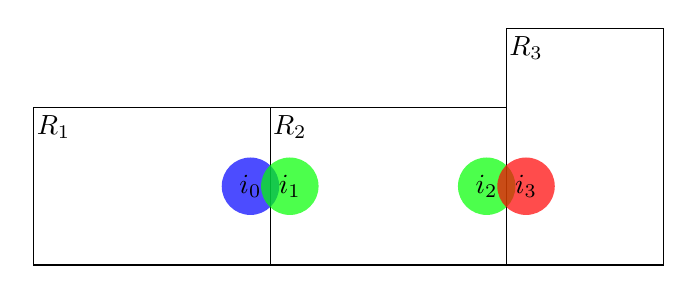
\begin{tikzpicture}[scale=0.5]

\draw  (0,0) rectangle (4,6);
\node at (0.5,5.5) {$R_3$};

\draw  (0,0) rectangle (-6,4);
\node at (-5.5,3.5) {$R_2$};

\draw  (-6,0) rectangle (-12,4);
\node at (-11.5,3.5) {$R_1$};

\node[rfid] at (-6.5,2) {$i_0$};
\node[rfid,fill=green] at (-5.5,2) {$i_1$};

\node[rfid,fill=green] at (-0.5,2) {$i_2$};
\node[rfid,fill=red] at (0.5,2) {$i_3$};

\end{tikzpicture}
\caption{Covering doors between rooms with antennas}
\label{rooms:fig:rooms}
\end{figure}

If an item first passes by $i_0$ and then $i_1$ we know that it has moved from $R_1$ to $R_2$ and likewise for the opposite direction.
If the object only passes by a single antenna (e.g. $i_0$) and loses the connection again, we know that it remains in $R_1$.

This method requires only knowledge about which room the item starts in to work.
The accuracy within a room is very granular as it is reduced to \textit{''in the room or not in the room''}.
However the system will always be able to correctly identify which room the object is located in, given that the initial room is known.